%%%%%%%%%%%%%%%%%%%%%%%%%%%%%%%%%%%%%%%%%%%%%%%%%%%%%%%%%%%%%%%%%%%%%%%%%%%%%%%%%%%%%%%%%%%%%%%%
 %
 % CSCI 1430 Final Project Report Template
 %
 % This is a LaTeX document. LaTeX is a markup language for producing documents.
 % Your task is to answer the questions by filling out this document, then to 
 % compile this into a PDF document. 
 % You will then upload this PDF to `Gradescope' - the grading system that we will use. 
 % Instructions for upload will follow soon.
 %
 % 
 % TO COMPILE:
 % > pdflatex thisfile.tex
 %
 % If you do not have LaTeX and need a LaTeX distribution:
 % - Departmental machines have one installed.
 % - Personal laptops (all common OS): http://www.latex-project.org/get/
 %
 % If you need help with LaTeX, come to office hours. Or, there is plenty of help online:
 % https://en.wikibooks.org/wiki/LaTeX
 %
 % Good luck!
 % James and the 1430 staff
 %
 %%%%%%%%%%%%%%%%%%%%%%%%%%%%%%%%%%%%%%%%%%%%%%%%%%%%%%%%%%%%%%%%%%%%%%%%%%%%%%%%%%%%%%%%%%%%%%%%
 %
 % How to include two graphics on the same line:
 % 
 % \includegraphics[width=0.49\linewidth]{yourgraphic1.png}
 % \includegraphics[width=0.49\linewidth]{yourgraphic2.png}
 %
 % How to include equations:
 %
 % \begin{equation}
 % y = mx+c
 % \end{equation}
 % 
 %%%%%%%%%%%%%%%%%%%%%%%%%%%%%%%%%%%%%%%%%%%%%%%%%%%%%%%%%%%%%%%%%%%%%%%%%%%%%%%%%%%%%%%%%%%%%%%%
 
 \documentclass[10pt,twocolumn,letterpaper]{article}
 
\usepackage{cvpr}
\usepackage{times}
\usepackage{epsfig}
\usepackage{graphicx}
\usepackage{amsmath}
\usepackage{amssymb}
\usepackage{booktabs}
\usepackage{microtype}
% From https://ctan.org/pkg/matlab-prettifier
\usepackage[numbered,framed]{matlab-prettifier}

\frenchspacing

% Include other packages here, before hyperref.

% If you comment hyperref and then uncomment it, you should delete
% egpaper.aux before re-running latex.  (Or just hit 'q' on the first latex
% run, let it finish, and you should be clear).
\usepackage[pagebackref=true,breaklinks=true,letterpaper=true,colorlinks,bookmarks=false]{hyperref}

\cvprfinalcopy
\def\cvprPaperID{****}
\def\httilde{\mbox{\tt\raisebox{-.5ex}{\symbol{126}}}}
\ifcvprfinal\pagestyle{empty}\fi

\begin{document}

%%%%%%%%% TITLE
\title{CSCI 1430 Final Project Report:\\Your project title}

\author{\emph{Urban Canopy Cover}: Elizabeth Zhang, Jenny Tan, Filip Kierzenka, Alexander Kamper\\
Brown University\\
}

\maketitle
%\thispagestyle{empty}

%%%%%%%%% ABSTRACT
\begin{abstract}
Expanding urban tree canopy cover is an important strategy for mitigating climate change, but estimating green space is an unresolved problem for spatial researchers. We aimed to reimplement Cai et al.’s approach using convolutional neural networks and compared it with a simpler architecture, DeepGreen. We also mapped and visualized the results for Providence’s canopy cover, and interpreted the model using the LIME explainer and Grad-CAM. We achieved a mean-squared error for the tree canopy cover estimation of 0.0909 for Cai et al.’s approach and 0.0969 for the DeepGreen approach.
\end{abstract}




%%%%%%%%% BODY TEXT
\section{Introduction}
Expanding urban tree canopy cover is one strategy for mitigating climate change, and a robust body of research indicates that green space is associated with a diversity of positive psychological and physiological effects for urban residents. Aside from carbon capture, enhancing wellbeing, and providing other ecosystem services, green spaces are beautiful and enhance the experience of urban dwelling. One method for estimating urban green space is by measuring tree canopy cover. However, quantifying urban tree canopy cover at scale is an unresolved problem for spatial researchers. Our goal was to replicate Cai et al.’s (2019)~\cite{Cai2019} novel approach and apply it to the city of Providence. Cai et al. (2019) applied two neural networks to street-level rather than aerial imagery in order to perform image segmentation and calculate greenness scores point-by-point along a city’s road network. The details and background research supporting this work are discussed in the method section. Assuming our process would be streamlined by referencing code published by the authors and MIT’s Senseable City Treepedia project, we defined several intermediate and stretch goals. First, we wanted to map and visualize our results in a way that would be intuitive for our audience and potential researchers interested in Providence’s urban canopy cover. Second, we wanted to compare the model’s performance against slightly different architectures. Finally, we wanted to interpret our model using the LIME explainer from homework 5 and Gradient-weighted Class Activation Mapping (Grad-CAM).


\section{Related Work}
As we concretized our project aims, we conducted an informal literature review on computer vision techniques for quantifying urban canopy cover. Based on our sampling, this body of research can be split primarily into two frameworks. First, there are approaches which attempt to segment canopy cover from satellite imagery and calculate it as a proportion of urban area. This idea is straightforward and falls within the standard set of techniques for geographic inquiry since the advent of geographic information systems (GIS) and the widespread availability of up-to-date, high resolution satellite images. The second approach proposes the deployment of UAVs, or drones, so that researchers can capture their own image data across whatever wavelengths and at whatever resolution their sensory equipment can capture (Seiferling, 2017)~\cite{Seiferling}. Research in this area is often coupled with research into machine learning approaches to autonomous flight so that data collection may be streamlined and standardized (Moreno-Armendáriz, Marco A et al., 2019)~\cite{Moreno}. This line of research breaks with the tradition of much modern geographic research and intrigues with its seeming orientation towards citizen science. Ignoring differences in granularity and access, however, these two approaches pose fundamentally the same engineering challenges for computer vision.

% Cite and discuss work that you used in your project, including any software used. Citations are written into a .bib file in BibTeX format, and can be called like this: Alpher et al.~\cite{Alpher04}. Here's a brief intro: \href{http://www.andy-roberts.net/writing/latex/bibliographies}{webpage}. \emph{Hint:} \$$>$ pdflatex \%docu, bibtex \%docu, pdflatex \%docu, pdflatex \%docu

\section{Method}

We utilized a combination of images from Google Street View and the Cityscapes dataset (~8000 images total). We used the original paper’s library to get the Google Street View images from five cities: Cambridge, Johannesburg, Oslo, Sao Paolo, and Singapore. The Cityscapes dataset originally had multi-class labels, and we converted the dataset to have binary labels for vegetation and non-vegetation. 80\% of the total images were used for training, and the other 20\% were used for validation. The images’ labels were their Green View Index - a pixel level average of canopy cover. GVI labels for Cityscapes were calculated using the “vegetation” mask in that dataset and the labels for GSV calculated via the original paper’s GVI library. GSV images and metadata for Providence were collected using our own modified version of the original paper's methods.


We re-implemented the convolutional neural network that was used in Cai’s approach. To reduce training time and computational power required, we used a ResNet50 architecture pre-trained on ImageNet and a dense classification head (Figure \ref{fig:dcnnmodel} and Table \ref{tab:dcnntable}). For the Deep Green Model, we used 5 convolutional blocks with a dense classification head that were not pretrained (Figure \ref{fig:dgreenmodel} and Table \ref{tab:dgreentable}). We decided on this model to determine how a decrease in model complexity would impact overall results.

We trained the model on the Google Street View images supplemented with the Cityscapes dataset. For gradient descent, we used mean squared error because we wanted to minimize the difference between the predictions and the labels. 

\begin{figure}[t]
    \centering
    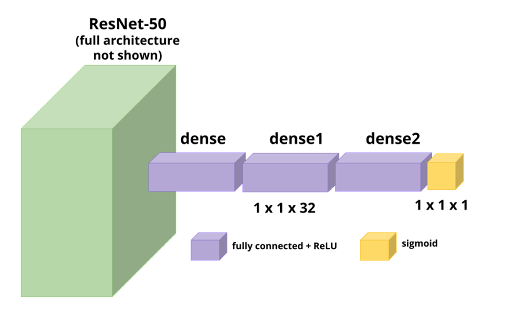
\includegraphics[width=\linewidth]{DCNN.png}
    \caption{Deep Convolutional Neural Net (DCNN) Architecture}
    \label{fig:dcnnmodel}
\end{figure}

\begin{table}
\begin{center}
\begin{tabular}{ l c }
\toprule
Hyperparameter & Value \\
\midrule
Batch size & 50 \\
Learning rate & 0.0001 \\
Momentum & 0.01\\
Optimizer & RMSProp\\
\bottomrule
\end{tabular}
\end{center}
\caption{Hyperparameters referenced from Cai et al.'s methodology (DCNN)}
\label{tab:dcnntable}
\end{table}

\begin{figure}[t]
    \centering
    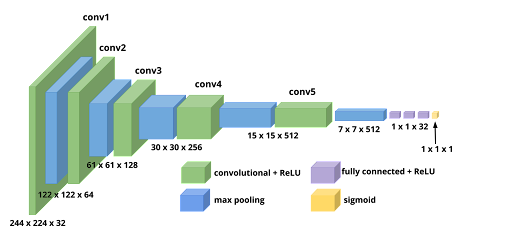
\includegraphics[width=\linewidth]{Deepgreen.png}
    \caption{DeepGreen Architecture}
    \label{fig:dgreenmodel}
\end{figure}

\begin{table}
\begin{center}
\begin{tabular}{ l c }
\toprule
Hyperparameter & Value \\
\midrule
Batch size & 50 \\
Learning rate & 0.01 \\
Optimizer & Adam\\
\bottomrule
\end{tabular}
\end{center}
\caption{Hyperparameters referenced from DeepGreen}
\label{tab:dgreentable}
\end{table}


\section{Results}

We reimplemented both the DCNN model  and the DeepGreen model, and were able to achieve a mean-absolute error of 0.0909 and 0.0969, respectively (Table \ref{tab:result1}). We found that the DeepGreen model’s performance was similar in terms of mean-squared error, and that the DeepGreen model was generally better than the DCNN model at distinguishing between vegetation and non-vegetation in the LIME explainer images. We have shown that a smaller, simpler architecture can still be effective at estimating the GVI. 

\begin{table}
\begin{center}
\begin{tabular}{c|c|c}
\toprule
Model & Lowest val. MAE & Epoch Achieved \\
\midrule
DCNN & 0.0909 & 13 \\
DeepGreen & 0.0969 & 18 \\
\bottomrule
\end{tabular}
\end{center}
\caption{Training results for both of our models.}
\label{tab:result1}
\end{table}

\begin{figure*}[t]
    \centering
    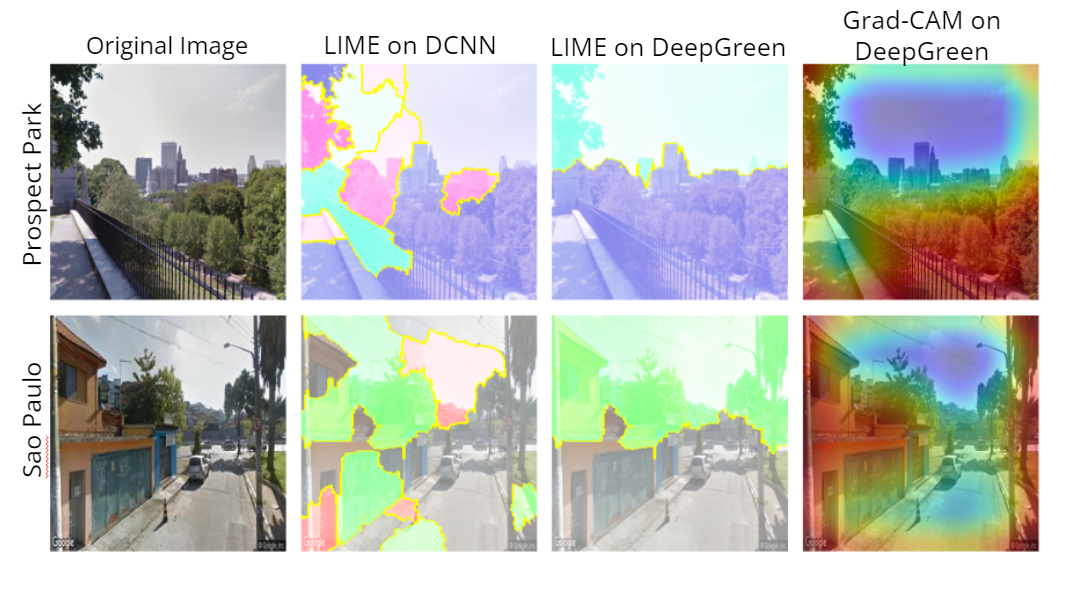
\includegraphics[width=0.8\linewidth]{lime_gradcam.PNG}
    \caption{LIME and GradCAM results for the DCNN and DeepGreen model}
    \label{fig:result2}
\end{figure*}

\begin{figure*}[t]
    \centering
    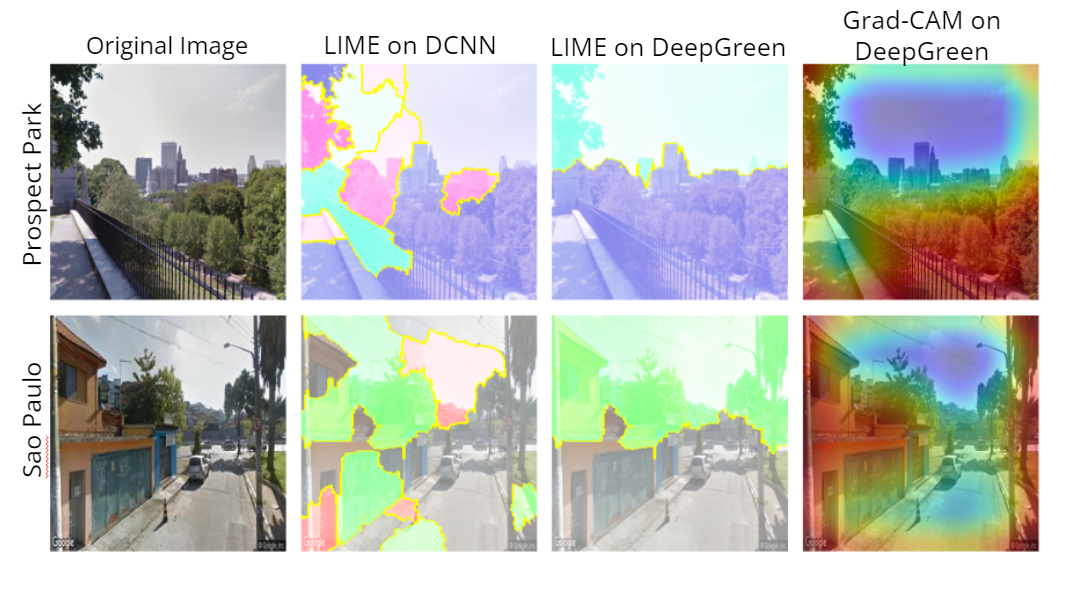
\includegraphics[width=0.8\linewidth]{lime_gradcam.PNG}
    \caption{LIME and GradCAM results for the DCNN and DeepGreen model}
    \label{fig:result3}
\end{figure*}

%-------------------------------------------------------------------------
\subsection{Technical Discussion}

Jun Yang and colleagues pioneered a novel approach to the quantification of urban canopy cover in 2009, proposing that instead of a top-down view of the city, researchers consider a pedestrian’s perspective to calculate what they termed a “Green View Index” (GVI) (Yang et al., 2009)~\cite{Yang2009}. Their approach was laborious, requiring researchers to manually collect and analyze images of the city on foot. Later, Xiaojiang Li et al., optimized this process by developing a program which could sample data from Google Street View (GSV). However, their automated technique for finding green vegetation was simplistic, simply calculating differences in the red, blue, and green bands of their dataset (Li et al., 2015)~\cite{Li2015}. Following an explosion of research in deep learning, Bill Cai collaborated with Li and a colleague in MIT’s Senseable City Lab to refine the GVI methodology using deep learning. They deployed a deep convolutional neural net (DCNN) to perform semantic segmentation on vegetation in GSV images, then used a second CNN with modified ResNet architecture to perform end-to-end learning on its outputs and calculate a GVI score for each coordinate at which the image was sampled.

We were able to achieve a mean-absolute error of 0.0909 from Cai et. al.’s model after 13 epochs. This was higher than the mean-absolute error described in the paper, which was 0.0467. This could be due to a difference in hyperparameters used in training, since the paper did not specify them. Additionally, we were able to achieve a mean-absolute error of 0.0969 using the DeepGreen model after 18 epochs (Table \ref{tab:result1}).

The DeepGreen model was better at classifying vegetation. In the images generated by the LIME explainer, we can see that the vegetation is marked, but other non-vegetation objects that were green in color were ignored. This did not seem to be the case in the DCNN model, as the DCNN highlighted a green garage door in the Sao Paulo test image (Figure \ref{fig:result2}). However, for the DeepGreen model, there was a significant difference between the LIME and GradCAM results. The LIME image for the Sao Paolo image shows the correct classification of vegetation, but the GradCAM image marks the buildings as more important than the vegetation. We were surprised by this disagreement, but it may be a matter of interpretation. GradCAM's "hot zones" refer to regions which, in the last CNN layer, increase the outputted value - it's possible that the overall values were generally too high before the final layer, and so the final CNN layer was reducing the value because of the vegetation. This would explain why the region with visible vegetation were blue in the GradCAM results.


%-------------------------------------------------------------------------
\subsection{Societal Discussion}

Research in political ecology and related disciplines has consistently shown how urban green spaces are distributed inequitably according to socioeconomic factors and legacies of structural racism. Heynens et al., (2006), performed a case study in Milwaukee, Illinois and found that canopy cover was correlated positively with both median household income and non-Hispanic white residents, demonstrating how richer, white residents had greater access to the psychological and physiological benefits of green space as compared to poorer, nonwhite residents (Heynens et al., 2006)~\cite{Heynen2006}. Urban tree canopy hence falls under the larger issue of urban environmental inequality and environmental justice more broadly.  

We received five points of feedback on the societal implications of our project through the SRC peer critique. They are outlined below, accompanied by our response to each.

1. The Street View car does not pass through all city streets, so that there are some
remote places that may be ignored, which is unfair to the people who live there.

This is true, but we also establish a sampling method of every 20 meters for computational efficiency so we acknowledge at the outset that this is not the most high resolution method possible for calculating urban canopy cover. One possible avenue for future research would be to set up our own street view data collection system with a mounted camera on a bike or car. Alternatively, cross-referencing our output with models using satellite or drone imagery could help address these blindspots in our data.

2. The privacy of others may be violated when getting the street view, because people
generally do not notice the street view car passing by them.

GSV is a legal project and takes measures to blur personally identifiable information like faces and license plates. Because the model outputs a greenness score which can then be mapped back onto the city, images of people will never show up in the outputs of our project. 

3. The cities chosen are among the more developed areas. Calculating tree canopy
area only in developed cities may affect the equity of development in different
areas.

Our aim is actually to apply this model to Providence, a relatively small city which wasn’t included in the set of global cities the Treepedia project included in their publications. We’ve discussed the possibility of continuing this work outside the scope of this class and considered creating a web app or some documentation that will make it easier for people without a programming background to create urban canopy cover maps of their own cities.

4. The data obtained by using only street view vehicles can only obtain data on the
tree canopy around the driveways, but some walkways or large green areas where
there are no driveways, these data will not be obtained, thus giving a bias to the
overall data correctness.

We sample images from a city (in this case Providence) by placing points every 20m on all roads, then querying the GSV API for panoramic images at those points. So its true that our method is somewhat constrained to roads. However, many parks and other green spaces are bordered by streets so we’d expect them to contribute to the greenscore of the city. Once again, cross-referencing our output with models using satellite or drone imagery could help remedy this issue.

5. Some cities will have a higher percentage of evergreen trees in all seasons, and
some cities will have trees that lose all their leaves in the fall. If these differences
are not differentiated, they may bias the correctness of the results.

During preprocessing we select images only from seasons where trees are green, which resolves this issue. However, there is merit to the fact that some urban areas are greener for longer periods of the year than others. This temporal component is not something we consider in the green score but perhaps could be an avenue for future research.


%------------------------------------------------------------------------
\section{Conclusion}

In the future, more research can be done to experiment with various kinds of architectures in order to improve the accuracy of estimating the GVI. Additionally, creating more mappings of the GVI in various geographic locations could be of interest to potential researchers who are interested in urban tree canopy cover. In the early stages of our project we discussed potentially converting our work into a web application that researchers and interested individuals could use to easily enter their location of interest and extract a set of green view indices for research. Visually this could be made more beautiful and engaging for non-academic users by embedding interactive web maps that would visualize GVI for the area of interest and have multiple toggle-able layers so the user could reference GVI against environmental justice factors like household income, race, and relevant health outcomes. Ultimately, we didn’t have time for this component and there remained a few bottlenecks that would need to be resolved before moving forward. Namely, due to lack of experience with the Google Streetview API, our code for collecting images and metadata behaved erratically for no apparent reason. Addressing this kink in the city choice, to point creation, to green view calculation and mapping pipeline would be a critical first step toward making this project into a potentially useful research tool. 

{\small
\bibliographystyle{plain}
\bibliography{ProjectFinal_ProjectReportTemplate.bib}
}

\section*{Appendix}

\subsection*{Team contributions}

Please describe in one paragraph per team member what each of you contributed to the project.
\begin{description}
\item[Person 1] Lorem ipsum dolor sit amet, consectetur adipiscing elit, sed do eiusmod tempor incididunt ut labore et dolore magna aliqua. Ut enim ad minim veniam, quis nostrud exercitation ullamco laboris nisi ut aliquip ex ea commodo consequat. Duis aute irure dolor in reprehenderit in voluptate velit esse cillum dolore eu fugiat nulla pariatur. 
\item[Person 2] Lorem ipsum dolor sit amet, consectetur adipiscing elit, sed do eiusmod tempor incididunt ut labore et dolore magna aliqua. Ut enim ad minim veniam, quis nostrud exercitation ullamco laboris nisi ut aliquip ex ea commodo consequat. Duis aute irure dolor in reprehenderit in voluptate velit esse cillum dolore eu fugiat nulla pariatur.
\item [Person 3] Lorem ipsum dolor sit amet, consectetur adipiscing elit, sed do eiusmod tempor incididunt ut labore et dolore magna aliqua. Ut enim ad minim veniam, quis nostrud exercitation ullamco laboris nisi ut aliquip ex ea commodo consequat. Duis aute irure dolor in reprehenderit in voluptate velit esse cillum dolore eu fugiat nulla pariatur. 
\item [Filip] I was responsible for getting the model training functionality working. I worked with Lizzy to write the training code, figure out how to best setup our datasets, and connect our model to that training code. I also did some work on the data side with Alex and Jenny; mainly helping to collect the Providence images via the GSV API, helping formating the data for prediction with our model, and format the models' output. I collected the images and did some writing for the results and methodology sections of the poster. 
\end{description}

\end{document}
